\section{问题三：连续通信约束下的运输与中继协同}
\subsection{问题分析}
\subsubsection{问题二与问题三的依赖关系}
问题三在运输可行性的基础上增加“任务全过程保持通信”的要求。通信需求不是服务区上的静态属性，而是随运输无人机位置和时间变化的轨迹属性；中继无人机也不是固定基站，它需要提前准备、飞抵候选点、完成建链，并在运输任务结束后返航和补能。因此，问题二提供的组批与路线只能作为运输侧候选，只有加入中继可达性、在位时段和资源周转后，才能判断联合方案是否真正可执行。

本文保留问题二的22条路线作为已通过硬时限与能量验证的候选，并在该候选上调整开始时刻、组织波次和配置中继。这样做能够清楚分离“运输方案本身是否可行”和“为了连续通信需付出多少等待与能量代价”，也便于沿用80箱唯一覆盖证据。相应局限是没有重新枚举所有组批、访问顺序和机型组合，因此所得结果是联合可行方案和当前搜索范围内的上界，而不是原问题完整联合决策空间中的全局最优解。

\subsubsection{时空耦合与主要难点}
连续通信至少包含四个层次。第一，链路必须双向可用，控制指令下发与状态回传任一方向不足都不能视为可通信；第二，地形遮挡只增加附加损耗，是否中断仍需与链路预算比较；第三，中继模式要求“运输机—中继”和“中继—网关”两条链路在同一时刻同时成立；第四，运输轨迹上的每一时刻都必须被直连或某架实际在服中继覆盖。

其计算难点在于，离散采样点全部可用并不能排除相邻样本之间的短时断链。山地视线关系还可能在航段经过像元边界时发生变化，使传播损耗并非仅由端点距离决定。故本文把固定步长采样用于候选筛选和独立复核，最终可行性由连续区间证书判断。

\subsubsection{输出目标与评价次序}
联合方案需要输出运输开始时刻、中继悬停点与服务区间、实体中继机和能源组件、每段通信方式、联合完成时间及总能耗。评价时首先要求31个硬时限箱不违约、每条运输轨迹连续通信、各类资源区间不冲突；在此基础上再比较一般物资迟到、联合完成时间、中继能耗和中继架次数。最小链路余量作为稳健性诊断指标单独报告，不用平均余量掩盖局部薄弱点。

\subsection{通信可用性模型}
\paragraph{双向链路预算}
固定网关G01位于O01，通信端点海拔由地面海拔与天线离地高度确定；运输端点随爬升、巡航、下降和交接阶段变化。接收门限为灵敏度与衰落裕量之和，附件中相应值为
\begin{equation}P_{th}=P_{sens}+M=-98+8=-90\ \mathrm{dBm}.\end{equation}
对通信方向$a\to b$，允许传播损耗为
\begin{equation}
L_{a\to b}^{max}=P_t^a+G_t^a+G_r^b-L_{sys}-P_{th}^b,\qquad
L_{ab}^{max}=\min(L_{a\to b}^{max},L_{b\to a}^{max}).
\end{equation}
两个方向取小值，是因为指令下发与状态回传均须可用。将附件对应接口参数代入，可得运输机—网关、运输机—中继和中继—网关的双向预算分别为122、116和126 dB。这些是设备参数推导的门限，不是某条实际航迹的通信余量。

设$D_{ab}(t)$为端点三维直线距离，单位km；频率$f$以MHz计，附件2.4 GHz对应2400 MHz。自由空间损耗常数及单位换算采用ITU-R P.525口径\textsuperscript{\cite{ITUP525}}；山地空地链路还需显式考虑视距与地形遮挡\textsuperscript{\cite{Feng2006,Zeng2016}}。传播损耗为
\begin{equation}
L_{ab}^{path}(t)=32.45+20\log_{10}f+20\log_{10}D_{ab}(t)+L_{obs}\beta_{abt}.
\end{equation}
其中$L_{obs}=10$ dB，遮挡变量由三维视线与沿途DEM比较确定。系统损耗已在预算侧扣除，不能在传播损耗侧再次扣减。定义
\begin{equation}
A_{ab}(t)=\ind\{L_{ab}^{path}(t)\le L_{ab}^{max}\},\quad
M_{ab}^{link}(t)=L_{ab}^{max}-L_{ab}^{path}(t).
\end{equation}
遮挡增加损耗，但不必然导致链路中断；最终仍须比较预算门限。

\paragraph{合法拓扑与全时段服务}
图\ref{fig:q3-topology}给出题目允许的两种通信方式。直连不可用时，可以经同一架中继完成接入和回传，不允许通过多架中继接力跳转。
\begin{figure}[htbp]\centering
\begin{tikzpicture}
\node[block,text width=2.5cm] (t) at(0,0){运输无人机};
\node[block,text width=2.5cm] (r) at(5,0){在服中继};
\node[block,text width=2.5cm] (g) at(10,0){固定网关G01};
\draw[edge,<->](t)--node[above,font=\small]{接入链路}(r);
\draw[edge,<->](r)--node[above,font=\small]{回传链路}(g);
\draw[edge,<->](t.south)--++(0,-1.1)--node[below,font=\small]{直连链路}(10,-1.6)--(g.south);
\node[font=\small,align=center] at(5,1.4){中继模式要求接入与回传同时可用\\拓扑示意，不表示实际点位或覆盖范围};
\end{tikzpicture}
\caption{直连与单中继通信拓扑示意}\label{fig:q3-topology}
\end{figure}

令$\mathcal T_r$为运输架次需要保障的全部飞行与交接时刻，$I_h^{srv}$为中继$h$的在服区间。对任意$t\in\mathcal T_r$，要求
\begin{equation}
A_{rG}(t)=1\quad\text{或}\quad
\exists h:\ t\in I_h^{srv},\ A_{rh}(t)=1,\ A_{hG}(t)=1.
\label{eq:continuous}
\end{equation}
输出时优先标记直连；非直连时选择一架满足条件的中继，保证每时刻只有一个实际保障指派。允许多个中继在物理上可用，但不能由此把同一运输区间同时计作多项必要保障任务。

\subsection{中继任务与资源模型}
\paragraph{候选悬停点与飞行过程}
候选悬停点$p$须在DEM内，海拔为$H_p^R=H_p^{DEM}+h_p^{AGL}$，且$0<h_p^{AGL}\le300$ m。中继出航巡航海拔还要覆盖终点悬停海拔：
\begin{equation}
H_{O01,p}^{c}=\max\left(\max_{c\in\mathcal C_{O01,p}}H_c+50,\ H_p^R\right).
\end{equation}
出航按爬升、水平巡航、必要下降计算，返航同理。中继从准备开始到建链完成的时刻依次为
\begin{align}
\tau_h^{dep}&=s_h+t_R^{prep},&
\tau_h^{arr}&=\tau_h^{dep}+t_{O01,p}^{fly},\\
\tau_h^{link}&=\tau_h^{arr}+t_R^{link},&
\tau_h^{ret}&=\tau_h^{end}+t_{p,O01}^{fly}.
\end{align}
只有在$[\tau_h^{link},\tau_h^{end}]$内才能提供保障。总能耗写为
\begin{align}
E_h^{fly}&=\frac{P_R^{cr}}{3600}\left(\frac{d_{O01,p}}{v_R^{cr}}+\frac{d_{p,O01}}{v_R^{cr}}\right)
+\frac{m_Rg_0(h_{O01,p}^{+}+h_{p,O01}^{+})}{3.6\times10^6\eta_R^{up}},\\
E_h&=E_h^{fly}+\frac{(P_R^{hover}+P_R^{com})(\tau_h^{end}-\tau_h^{arr})}{3600}
\le(1-\rho_R)E_R^{use}.\label{eq:relay-energy}
\end{align}
功率以kW计，故时间需除以3600。这里把建链期间按悬停及通信功率计入能源消耗，明确计费从抵达开始，而服务可用从建链完成开始。

\paragraph{实体机、能源组件与可用区间}
中继实体机占用$[s_h,\tau_h^{ret}+t_R^{turn})$；能源组件占用任务及返航后充电区间。两架中继机和六组能源组件均按实体编号分配，在同一波次内也须逐一预占，不能让多个任务同时选中尚未更新状态的同一资源。

\subsection{候选覆盖与联合调度方法}
\paragraph{离线选点与方案固化}
先将运输任务展开为分段线性三维轨迹，识别直连不足的时空位置。独立选点脚本在服务区邻域、航段附近和DEM高点形成候选悬停集合，并按5~s黑障样本筛选越界、回传不足和往返能量不可行的点。搜索得到的六个点位与七个运输波次随后固化到主求解器；离散样本仅用于离线筛选，最终仍按式\eqref{eq:continuous}验证整段时间。

离线候选点生成兼顾覆盖与代价。服务区邻域点有利于保障下降和交接阶段，航段投影附近点有利于缩短运输机—中继距离，局部高点则有利于改善中继—网关视距。对于每个候选点，先检查DEM范围和离地高度，再检查中继到网关的回传预算，最后计算出航、返航和最长可悬停时间。主求解器只接收离线筛选后固定的P1A、P1B、P2A、P2B、P3A和P4B六个点位，并显式检查输入是否为22个运输架次。

\paragraph{覆盖关系与运输波次}
将每条运输轨迹划分为直连区间和需要中继的区间。离线搜索把22个运输任务组织为W1--W7七个固定波次，并为每个波次配置一个或两个上述点位；中继须在波次首个需求时刻之前完成建链，并持续到最后一个实际保障区间结束。主程序依次执行这些固定波次，由资源事件仿真分配两架中继机和六套能源组件，再对全部链路实施连续认证。故该程序证明的是固化方案可行，而非在线贪心选点的全局最优性。

运输波次并非越集中越好。集中可以提高一次中继在位期间的覆盖利用率，但也可能需要多个中继点同时在服，并推迟部分运输任务；分散则降低并发资源，却增加重复准备、飞抵和返航。本文在硬时限和连续覆盖成立的前提下，以一般物资迟到、联合完成时间、能耗和架次数依次评价这种取舍。

图~\ref{fig:q3-flow}概括问题三的覆盖筛选、资源排程与连续认证闭环。离散样本只负责加速候选筛选；任何未通过连续区间认证的方案都必须返回选点或波次调整步骤。
\begin{figure}[H]\centering
\begin{tikzpicture}[node distance=6mm]
\node[block,text width=7.6cm](traj){读取运输路线与时序\\展开爬升、巡航、下降和交接轨迹};
\node[block,text width=7.6cm,below=of traj](blind){计算直连状态\\提取非直连时空区间};
\node[block,text width=7.6cm,below=of blind](candidate){读取离线筛选的六个悬停点\\核验点位、回传和往返能量};
\node[block,text width=7.6cm,below=of candidate](cover){执行固化的W1--W7运输波次\\分配中继机与能源组件};
\node[block,text width=7.6cm,below=of cover](cert){连续区间证书与0.5~s加密采样\\复核链路、能量和资源占用};
\node[block,text width=7.6cm,below=of cert](output){输出联合时序、通信分段、链路余量\\联合完工时间与总能耗};
\draw[edge](traj)--(blind);\draw[edge](blind)--(candidate);\draw[edge](candidate)--(cover);
\draw[edge](cover)--(cert);\draw[edge](cert)--node[right,font=\small]{通过}(output);
\draw[edge](cert.east)--++(1.2,0) node[right,font=\small]{未通过} |- (candidate.east);
\end{tikzpicture}
\caption{问题三运输—中继协同求解与认证流程}\label{fig:q3-flow}
\end{figure}

\paragraph{中继任务阶段与联合目标}
图\ref{fig:q3-phase}把最终选中的11个中继架次拆为准备、飞抵与建链、在位保障以及返航三个阶段。不同架次的在位时长差异明显，因此各架次均按实际保障区间核算能耗和资源占用。
\begin{figure}[htbp]
  \centering
  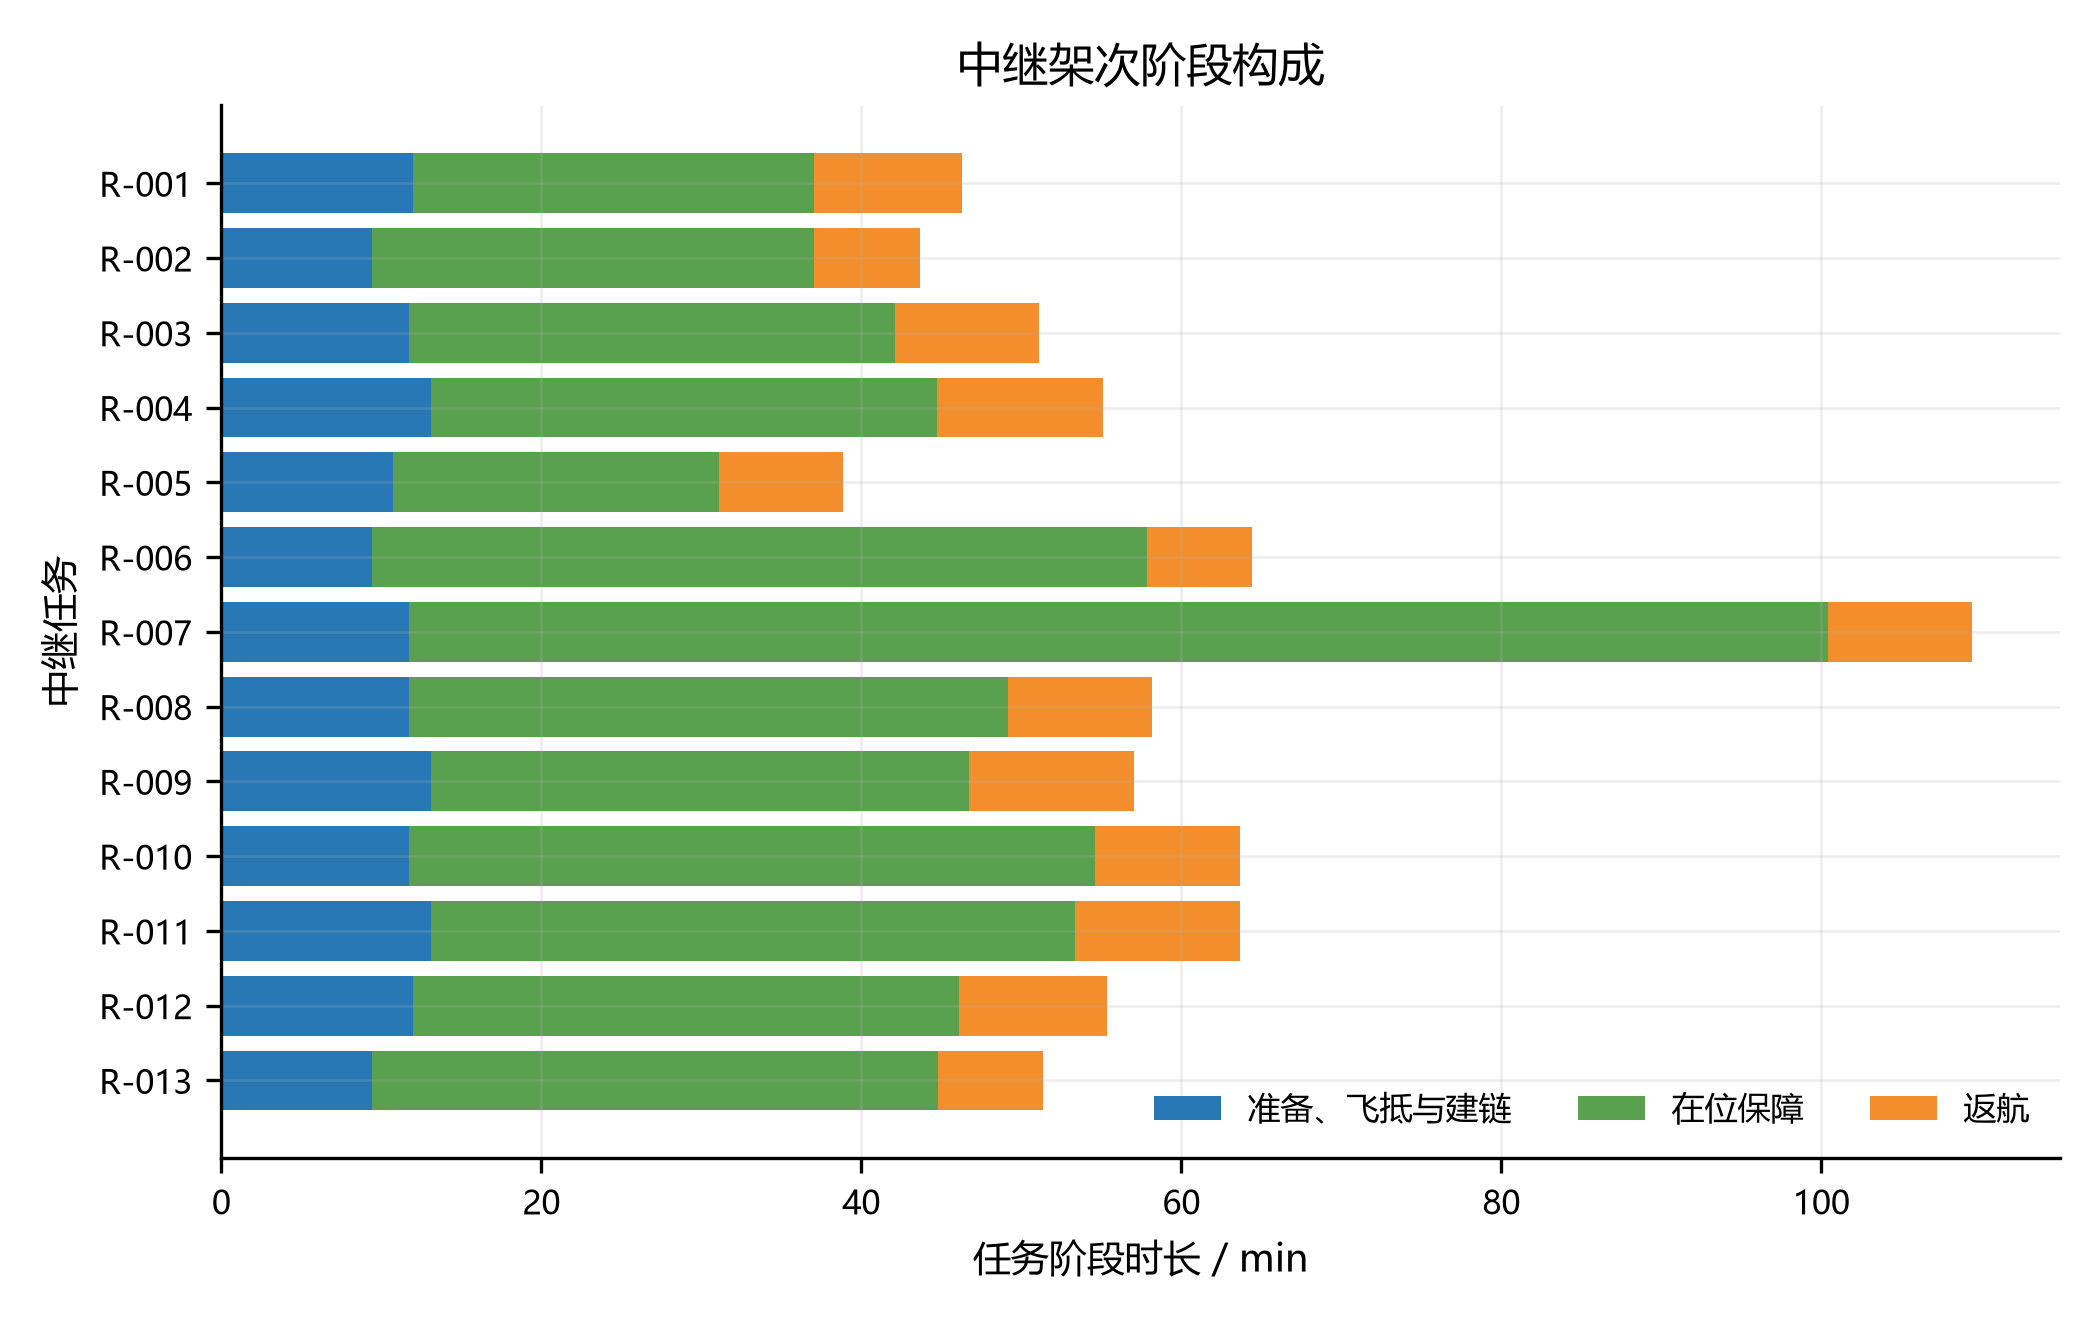
\includegraphics[width=0.92\textwidth]{figures/q3_q4/raw_q3_relay_phase_duration.png}
  \caption{中继架次的阶段时长构成}
  \label{fig:q3-phase}
\end{figure}

联合候选方案采用硬截止优先组织运输批次，并根据中继最早建链时刻、最长可服务时长和能源再可用时刻调整波次。比较指标为一般物资迟到、联合完成时间、总能耗和总架次，其中
\begin{equation}
C_{max}^{joint}=\max\!\left(\max_r\tau_r^{ret},\max_h\tau_h^{ret}\right),\quad
E^{joint}=\sum_rE_r+\sum_hE_h.
\end{equation}
完成时间取最后返航，不包含此后的充电及周转。硬时限与连续通信必须先满足；不能用较少的中继能耗补偿已发生的通信中断。

\subsection{连续性验证与联合调度结果}
\paragraph{连续区间认证方法}
固定时间网格不能排除相邻样本之间的短时中断。验证时，应在每个线性运动区间给出传播损耗上界：距离项在区间端点求上界，地形项采用扫掠视线与经过像元的关系获得保守判定；无法判定的区间进一步细分。区间达到细分阈值仍未被证明可用时，应标记为未通过证明，不将其自动视为可行，也不直接断言实际已经中断。

具体而言，先以轨迹的运动阶段端点、通信方式切换时刻和中继服务边界切分时间轴，使每个初始区间内端点运动均为线性。对直连候选，计算运输机到网关的距离上界和遮挡保守值；对中继候选，分别计算接入链路与回传链路的下界余量，并取二者较小值。若整个区间的服务余量下界非负，则该区间被认证；否则对半分割，直至找到可用证据或达到0.1~s阈值。达到阈值仍无法证明的区间按不可用处理，这一规则宁可拒绝边界方案，也不把数值不确定性误判为连续通信。

\paragraph{联合排程总体结果}
基于问题二的22条冻结路线，将任务按资源可行性和通信需求组织为7个波次。最终安排11个中继架次，使用2架中继无人机和5套能源组件，第6套能源组件保留备用。运输路线和运输能耗保持不变；为等待中继完成准备、飞抵和建链，运输完成时刻由问题二的$9643.106\ \mathrm{s}$延后到$23117.362\ \mathrm{s}$。最后一架中继于$23658.349\ \mathrm{s}$返航，因此联合完成时间为$6.572\ \mathrm{h}$。

\begin{table}[htbp]
  \centering
  \caption{问题三联合调度与连续通信的关键结果}
  \label{tab:q3-summary}
  \begin{tabular}{lrl}
    \toprule
    指标 & 数值 & 说明 \\
    \midrule
    运输架次/波次 & $22/7$ & 7个波次均配置中继 \\
    中继架次 & $11$ & 由2架中继机执行 \\
    实际使用能源组件 & $5$ & 库存为6套 \\
    通信分段数 & $68$ & 41段直连、27段中继 \\
    连续未解析区间 & $0$ & 22个架次均完成区间认证 \\
    0.5 s网格点/中断点 & $65532/0$ & 独立加密采样复核 \\
    最小保守链路余量 & $0.139703\ \mathrm{dB}$ & 出现在T005与T021 \\
    联合完成时间 & $23658.349\ \mathrm{s}$ & 取最后运输或中继返航 \\
    \bottomrule
  \end{tabular}
\end{table}

\paragraph{通信分段与双重验证}
连续区间证书把每段最小服务余量写为
\begin{equation}
M^{service}(t)=\max\left\{M_{TG}(t),\max_h\min\left[M_{TR_h}(t),M_{R_hG}(t)\right]\right\}.
\end{equation}
若采样余量减去区间变化上界后仍非负，则整段得到认证；否则继续二分。22个架次均未出现未解析区间；另以0.5 s步长检查65532个点，也未发现中断。表\ref{tab:q3-summary}汇总了连续区间认证与加密采样的结果。

图\ref{fig:q3-gantt}显示两架中继机在各波次之间交替执行，不存在机体占用重叠；能源组件的充电与复用由同一事件时间轴核算。图\ref{fig:q3-timeline}把68个通信分段展开，其中斜线区段表示实际使用中继。
\begin{figure}[htbp]
  \centering
  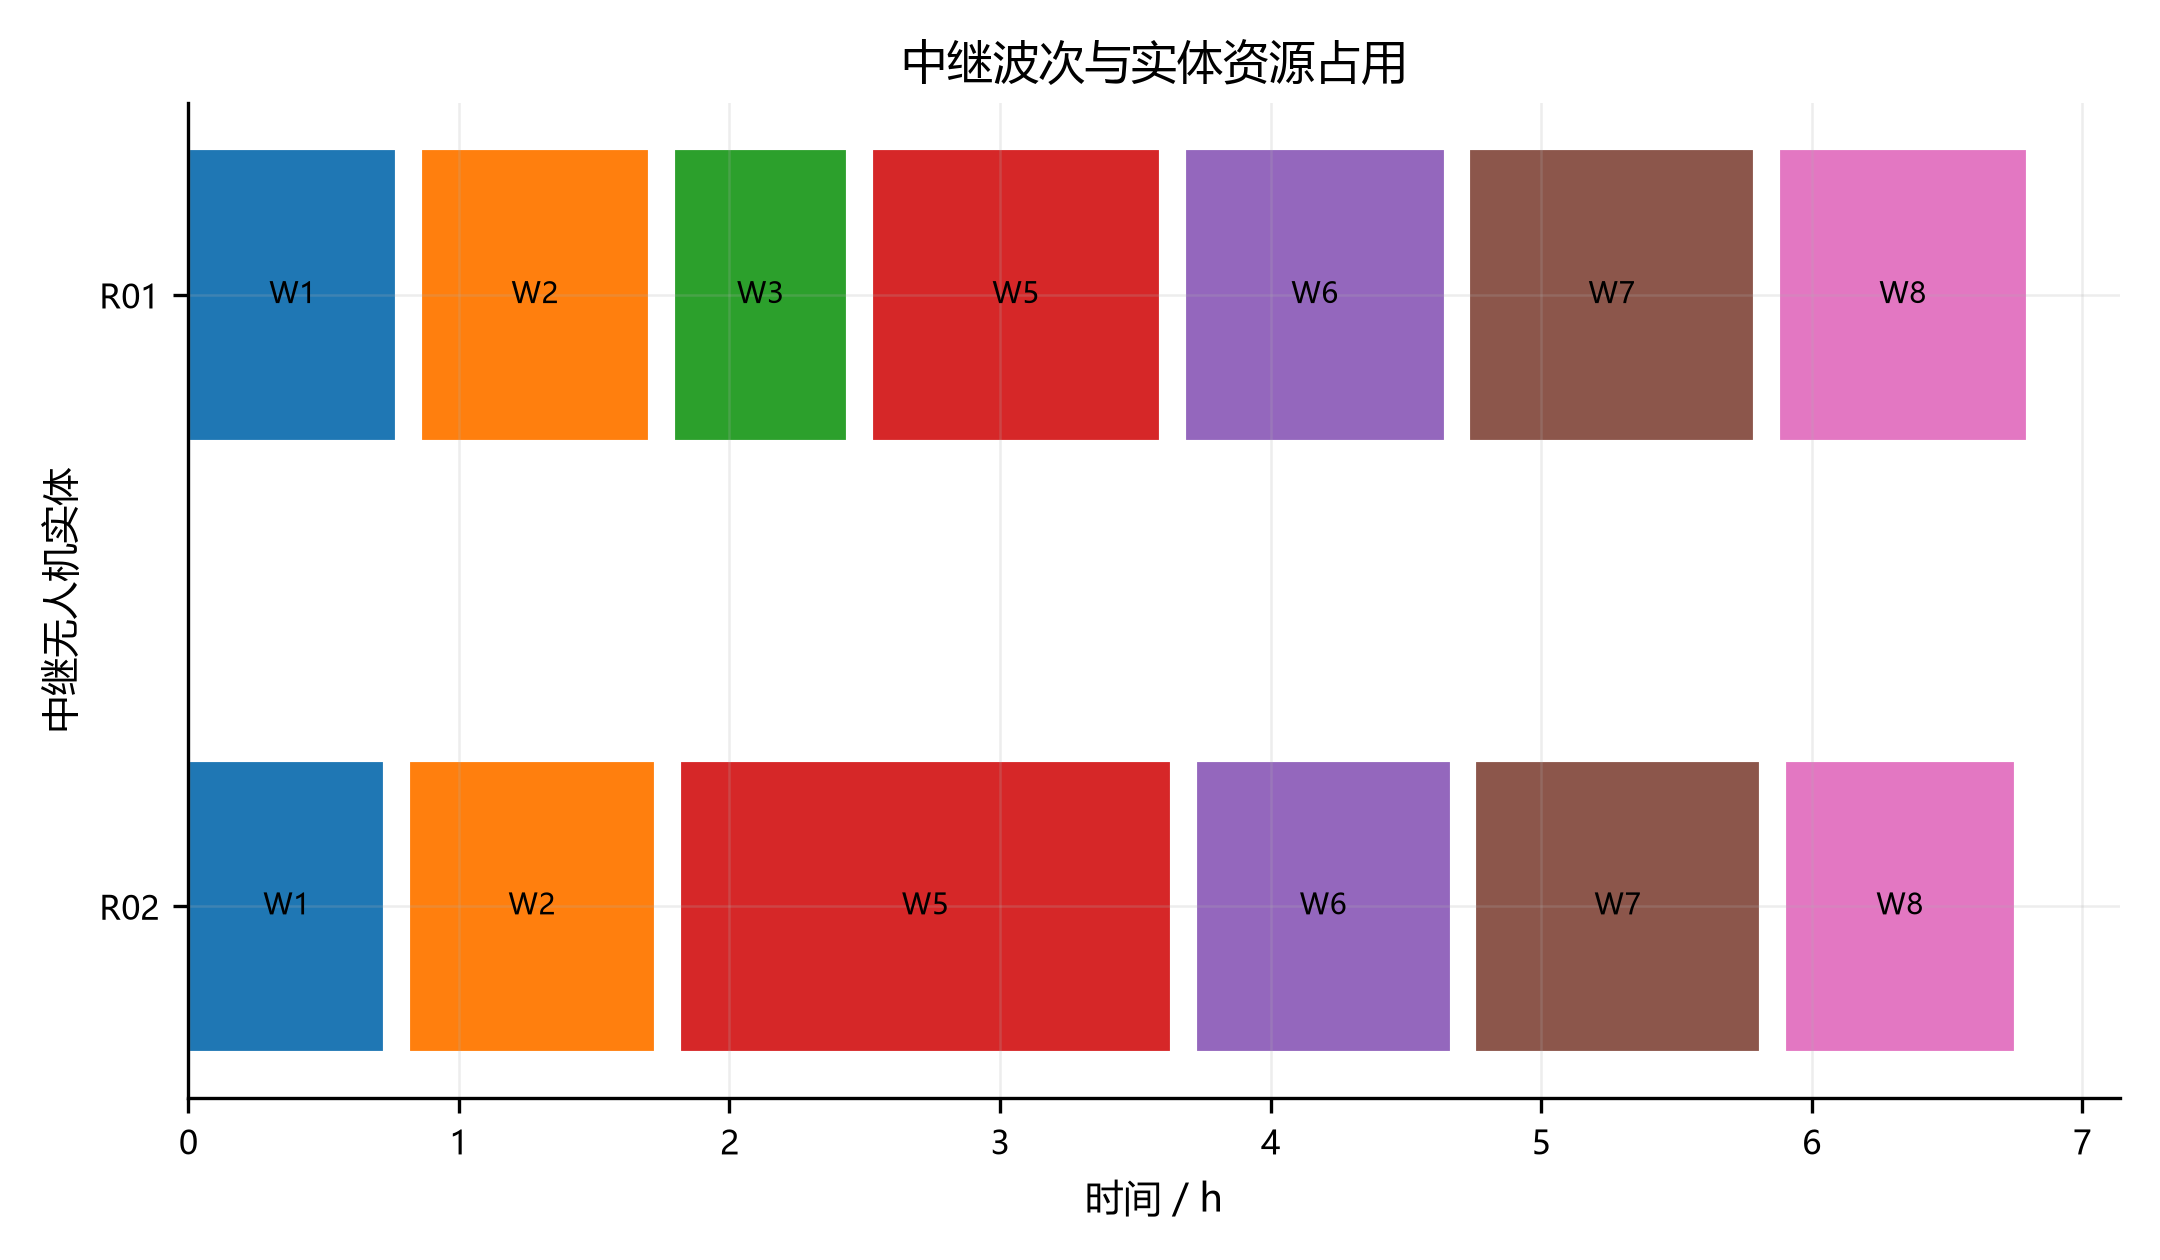
\includegraphics[width=0.92\textwidth]{figures/q3_q4/process_q3_relay_gantt.png}
  \caption{中继波次与实体资源占用时间轴}
  \label{fig:q3-gantt}
\end{figure}

\begin{figure}[htbp]
  \centering
  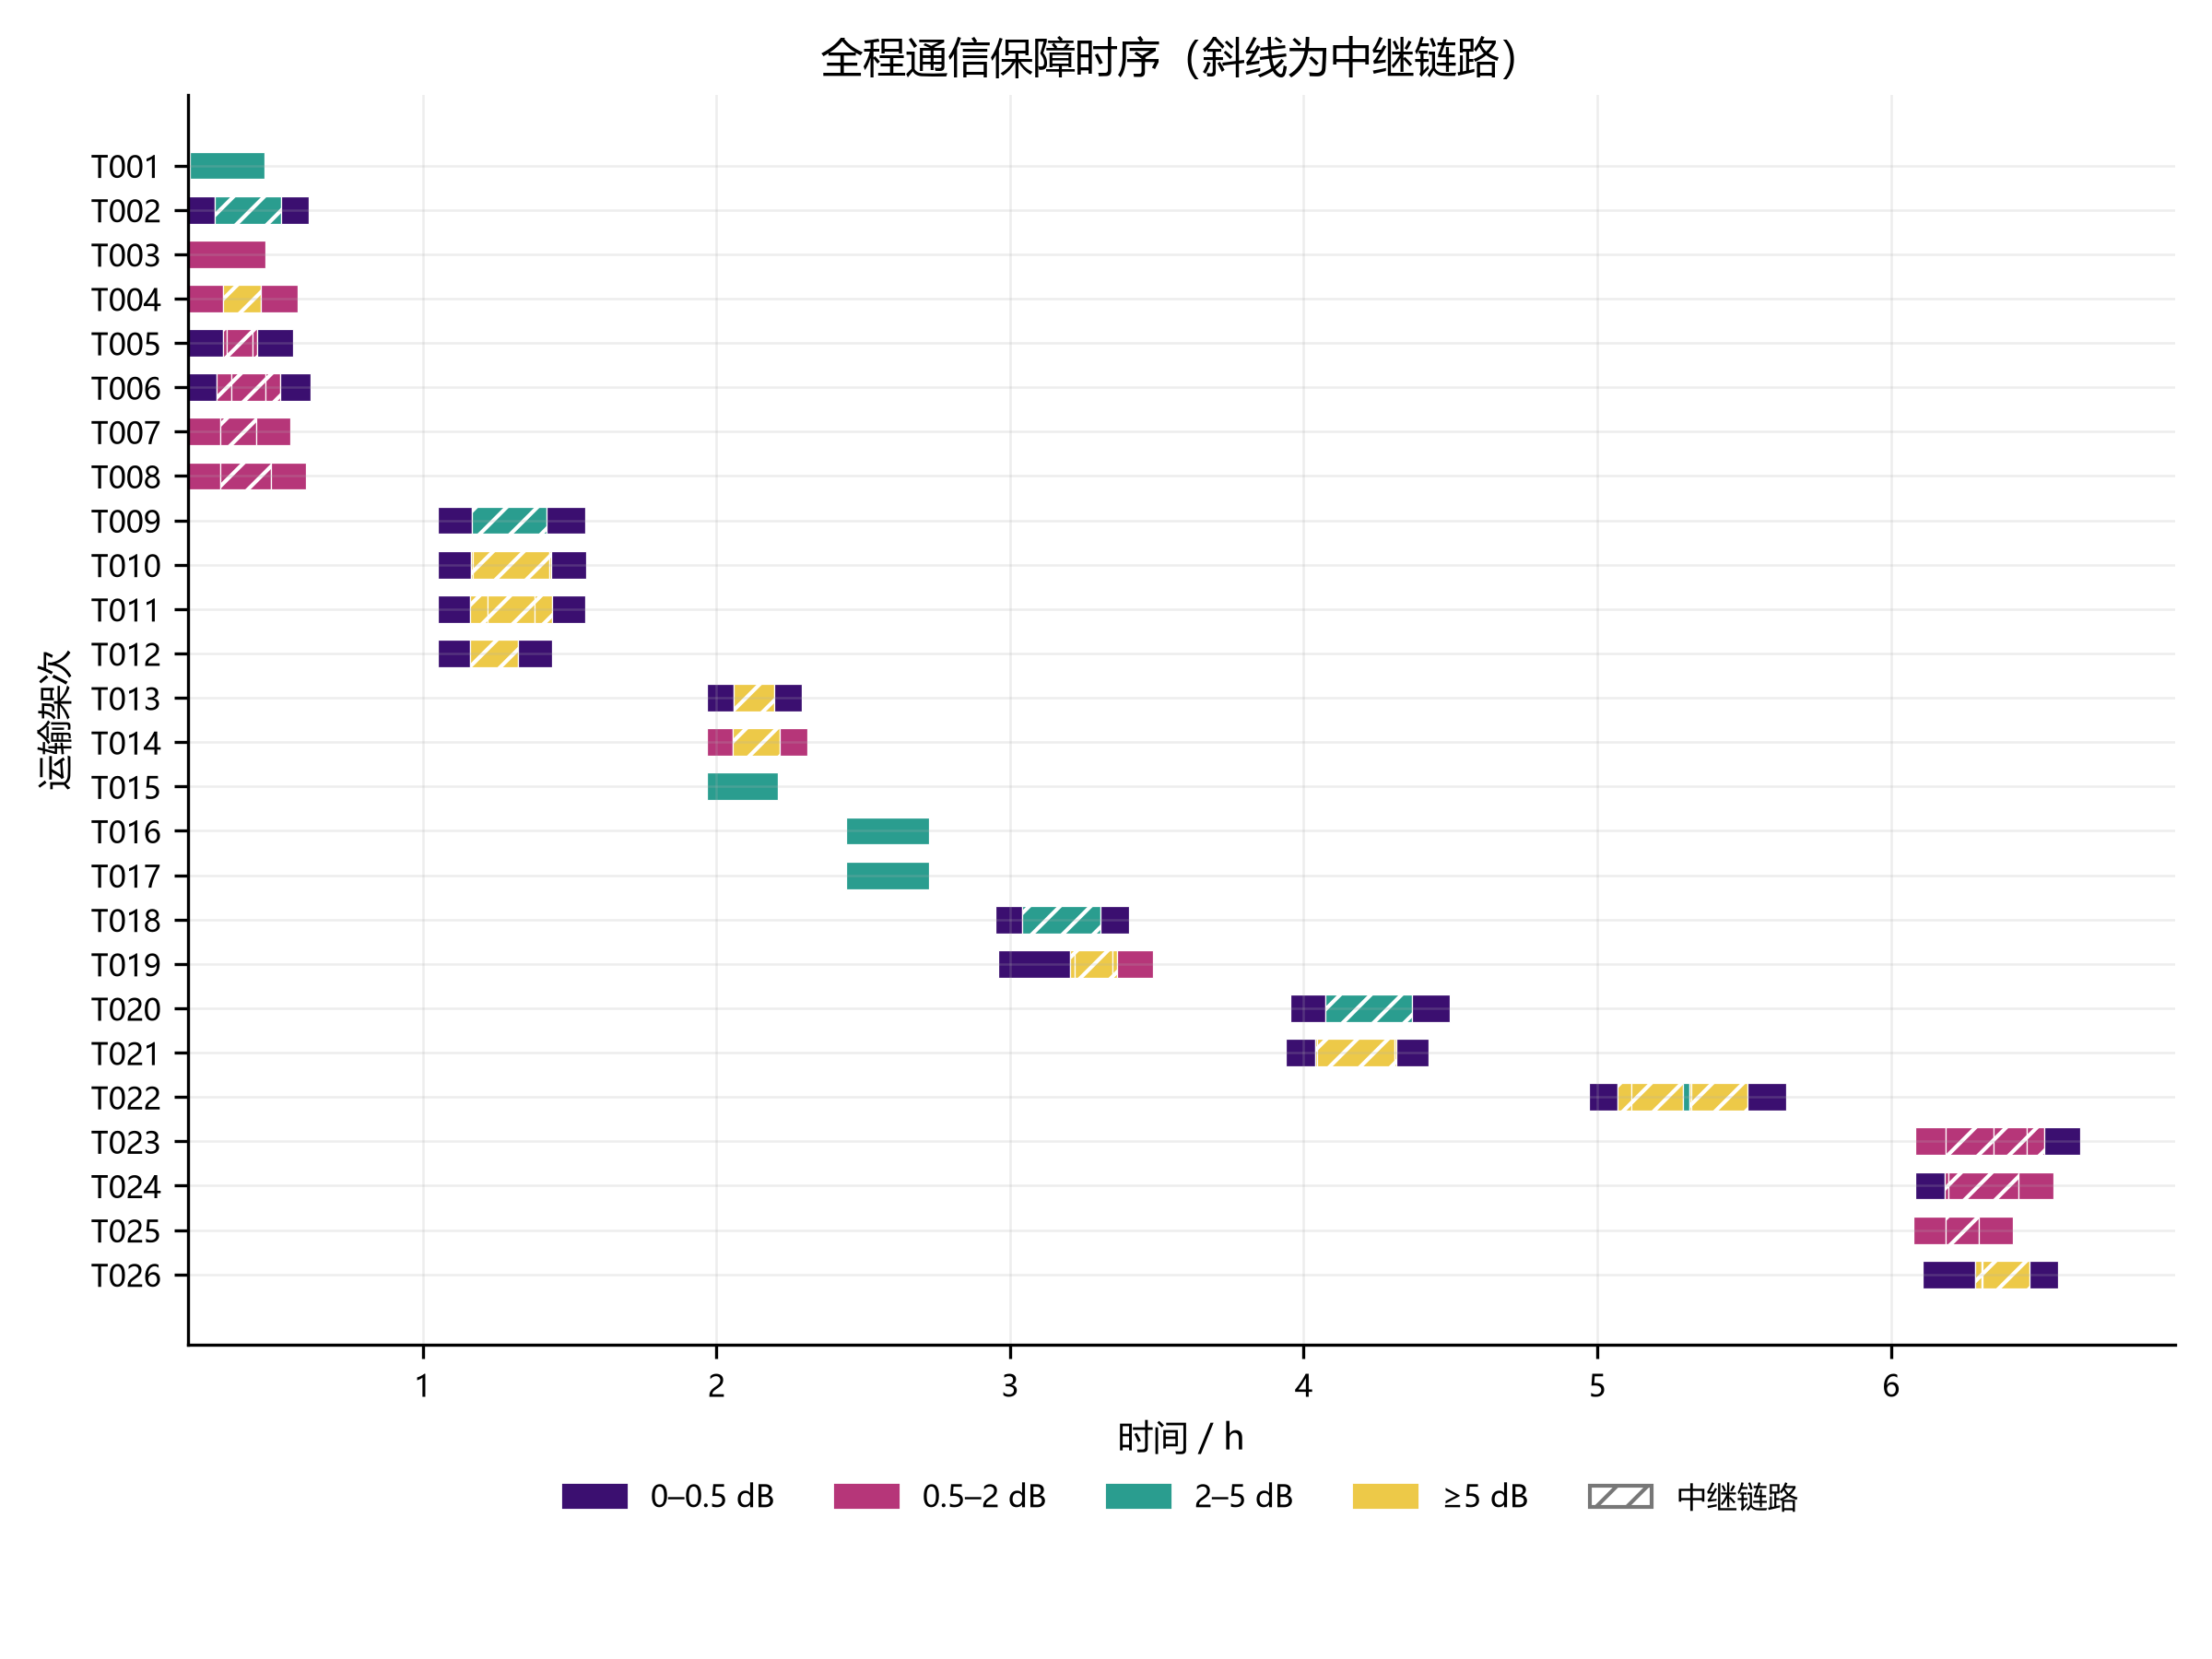
\includegraphics[width=0.98\textwidth]{figures/q3_q4/result_q3_communication_timeline.png}
\caption{22个运输架次的全程通信保障时序}
  \label{fig:q3-timeline}
\end{figure}

\paragraph{通信保障代价}
中继能耗为$9.495539\ \mathrm{kWh}$，与运输能耗$69.601587\ \mathrm{kWh}$相加得到
\begin{equation}
E^{joint}=69.601587+9.495539=79.097126\ \mathrm{kWh}.
\end{equation}
通信约束没有改变既定运输路线的飞行能耗，但波次平移使一般物资超期箱数由9箱增至32箱，$WTD$由38.787增至297.276。该结果表明，当前联合方案首先满足硬时限和连续通信，后续仍可在不改变路线的条件下压缩波次等待时间。

从增量角度看，通信保障增加了9.496~kWh能耗，占联合总能耗的12.0\%；联合完成时间相对问题二运输完成时间增加3.893~h。时间增量明显大于能量增量，说明当前方案的主要代价来自等待中继就位和波次协调，而不是中继飞行本身。优化空间因此更可能出现在波次起始时刻、候选点覆盖复用和中继资源衔接，而非单纯降低悬停功率。

\subsection{链路裕量诊断与实施边界}
\paragraph{附加损耗敏感性}
在已通过的连续证书上统一扣除附加链路裕量，可判断现有证书能否继续提供保证，结果见表\ref{tab:q3-margin}。附加裕量为0.1 dB时22个架次的原证书仍全部有效；提高到0.2 dB后仅16个架次保留原证书。这里的“未保留”表示需要重新搜索悬停点并重新认证，并不等同于已经发生通信中断。
\begin{table}[htbp]
  \centering
  \caption{附加链路裕量下的连续证书保留情况}
  \label{tab:q3-margin}
  \begin{tabular}{rrrr}
    \toprule
    附加裕量/dB & 保留证书架次 & 需重新认证架次 & 最差调整余量/dB \\
    \midrule
    0.0 & 22 & 0  &  0.140 \\
    0.1 & 22 & 0  &  0.040 \\
    0.2 & 16 & 6  & -0.060 \\
    0.5 & 8  & 14 & -0.360 \\
    1.0 & 4  & 18 & -0.860 \\
    2.0 & 3  & 19 & -1.860 \\
    \bottomrule
  \end{tabular}
\end{table}

\paragraph{工程解释与适用边界}
若实测后附加损耗超过0.1 dB，应重新搜索更高且合法的悬停点或增加靠近薄弱航段的候选点，而不能仅延长中继服务时间；后者无法改善由几何遮挡和链路预算造成的余量不足。

最小余量0.1397~dB表明当前方案在题设传播模型下可行，但通信稳健性偏紧。DEM只描述地形，未显式包含树木、建筑、降雨和小尺度多径；实际部署前应进行现场链路测量，并把测得的附加损耗重新代入连续认证。若现场要求更大的工程余量，还需要重新选点或增加中继，而不能把本题计算值直接视为飞行许可。
